\documentclass[12pt,letterpaper]{article}
\usepackage[utf8]{inputenc}
\usepackage[spanish,es-tabla]{babel}
\usepackage{amsmath}
\usepackage{amsfonts}
\usepackage{amssymb}
\usepackage{graphicx}
\usepackage[margin=2.5cm]{geometry}
\usepackage{hyperref}
\usepackage{float}
\author{Rodrigo Zaldivar Alanis}
\title{
    \vspace{-2cm}
    \begin{center}
        \Large \textbf{Universidad Nacional Autónoma de México} \\
        \vspace{0.2cm}
        \large \textbf{Facultad de Ciencias} \\
    \end{center}
    \vspace{0.5cm}
    \textbf{Implementación de Aceptación por Umbrales para el problema del Agente Viajero}
}
\date{\today}

\begin{document}

\maketitle

\begin{abstract}
El presente trabajo es un reporte acerca de mi implementación de Aceptación por Umbrales, una variante de la Heurística de Recocido Simulado, específicamente para la resolución del Problema del Agente Viajero (TSP) en su variante de Camino Hamiltoniano. Para el desempeño de la implementación, se diseñó un estudio experimental sobre la instancia de 150 ciudades ejecutando una muestra de 1000 semillas pseudoaleatorias. La mejor solución encontrada para dicha instancia fue de 0.139402 en un tiempo aproximado de 50s.
\end{abstract}

\section{Introducción}
El Problema del Agente Viajero (TSP, por sus siglas en inglés) es uno de los problemas de optimización combinatoria más estudiados, clasificado dentro de la categoría NP-Hard. Su premisa consiste en encontrar el ciclo hamiltoniano de menor costo que visite un conjunto de vértices exactamente una vez. Debido a la explosión combinatoria del espacio de búsqueda ($O(n!)$, que para una instancia de 150 ciudades es mucho más grande que el número de partículas en el universo observable), los métodos exactos resultan computacionalmente inviables para instancias de gran escala \cite{michalewicz2000}. 

Para evadir óptimos locales y obtener aproximaciones de alta calidad en tiempos polinomiales, se recurre a metaheurísticas de trayectoria. En esta práctica se implementa la Aceptación por Umbrales (\textit{Threshold Accepting}), un método que simplifica la regla probabilística del Recocido Simulado mediante un enfoque determinista para la aceptación de peores soluciones \cite{dueck1990}.

\section{Marco Teórico}
A diferencia del Recocido Simulado tradicional que evalúa la aceptación de un vecino peor $s'$ mediante una probabilidad $e^{-\Delta / T}$, la Aceptación por Umbrales propone que un empeoramiento es aceptado si y solo si la diferencia de costo $\Delta = f(s') - f(s)$ es menor o igual a un umbral $T$ (temperatura actual). 

El esquema de enfriamiento diseñado mantiene la temperatura constante durante un lote de evaluaciones. El algoritmo desciende a la siguiente temperatura ($T_{k+1} = \alpha T_k$) únicamente cuando se alcanza el equilibrio térmico en el vecindario local. Este estancamiento se detecta midiendo el costo promedio del lote anterior ($q$) contra el costo promedio del lote actual ($p$). Si la mejora no supera un valor mínimo $\epsilon$ ($q - p \le \epsilon$), se procede a enfriar el sistema. De esta manera, se evita caer en mínimos locales mediante la última solución aceptada. Que puede ser o no la mejor de su vecindario, pero esto permite explotar un gran número de soluciones porque se evita un acercamiento \textit{greedy}.

\section{Diseño}
El enfoque principal en cuanto al diseño fue desacoplar lo más posible la heurística de Aceptación por Umbrales del modelo de TSP en su variante de camino hamiltoniano. Para esto, el código se dividió en varios paquetes principales:
\begin{itemize}
    \item models\\
    Establece la conexión a la base de datos y ejecuta las consultas necesarias para obtener las coordenadas de las ciudades y la distancia entre estas.
    \item tsp\\
    Se encarga principalmente de modelar adecuadamente las instancias de TSP. Se encarga de construir una tabla con el peso de las conexiones entre las ciudades. A pesar del gran tamaño del número total de ciudades en la base de datos y de la dispersión de los índices de estas en las instancias, se optó por una matriz cuadrada, de tamaño máximo $(n=$índice máximo en la instancia + 1$)\cdot(n=$índice máximo en la instancia + 1$)$.
    Este paquete asimismo se encarga de obtener todas las distancias que no estén presentes en la base de datos, y la integra en nuestra matriz de ciudades, con una penalización, para forzar soluciones factibles.
    \item simulated\_annealing\\
    Este paquete implementa los algoritmos proporcionados de Aceptación por Umbrales: Aceptación por Umbrales, ProcesarLote, Temperatura Inicial, Búsqueda Binaria. Estos algoritmos operan sobre una interfaz \textit{Solution}. De esta manera obtenemos el desacoplamiento. Esta interfaz cuenta con dos métodos que deben implementarse: \texttt{Cost() float64} y \texttt{GetNeighbour() Solution}.
    \item tsp\_solver\\
    Implementa la interfaz \textit{Solution} al problema TSP mediante el struct \textit{travel\_solution}. Proporciona un struct \textit{instance} que contiene la matriz de adyacencias de la instancia y el generador de números pseudoaleatorios. También, en este paquete se ejecuta la heurística sobre el problema.
    \item cli\\
    Se encarga de obtener la semilla correspondiente mediante la bandera \texttt{-seed}. En caso de no ser proporcionada, se toma el valor por defecto 4. Lee la instancia mediante la entrada estándar, que se asume es una lista de números enteros separados por comas. También se ocupa de inicializar la base de datos, hacer las consultas correspondientes, y crear un objeto \textit{instance} para poder obtener una solución al problema.
\end{itemize}

\section{Implementación y Metodología}
La heurística fue programada en el lenguaje Go, priorizando la concurrencia y la eficiencia en el manejo de memoria.
\begin{itemize}
    \item \textbf{Mutación \textit{in-place} y Rollback:} En lugar de instanciar nuevas estructuras por cada evaluación, las permutaciones se alteran sobre referencias en memoria (punteros). Si un movimiento es rechazado, la función \texttt{RollBack()} deshace los cambios atómicamente, eliminando la carga del \textit{Garbage Collector}.
    \item \textbf{Parámetros Experimentales:} Se utilizaron lotes de 5,000 iteraciones por nivel térmico, un factor de enfriamiento $\alpha = 0.95$ y una tolerancia $\epsilon = 0.0001$. Se procesaron 1,000 semillas concurrentemente utilizando \textit{goroutines}.
\end{itemize}

\section{Desarrollo}
El desarrollo estuvo dividido en varias fases:
\begin{itemize}
    \item Implementación de la función de Costo y la modelación de la entrada.\\
    En esta fase se codificó el paquete \textit{tsp} y el manejo de instancias, así como el paquete \textit{simulated\_annealing}. Todo principalmente enfocado a desarrollar la función Costo para una permutación, respaldado por pruebas unitarias, definiendo además el struct \textit{travel\_solution}.
    \item Implementación de la función vecino:\\
    Se obtiene un vecino en tiempo constante, mediante un intercambio de índices en la permutación, se calcula el nuevo costo a partir de la solución original más la diferencia que las aristas de la nueva permutación genera, menos la diferencia que generaban las aristas de los índices antes de ser intercambiados. En esta fase, se validó esta función comparando su resultado contra el cálculo de costo completo de la permutación vecina.
    \item Implementación de la heurística\\
    Se implementaron los algoritmos de aceptación por umbrales y el algoritmo de procesamiento de lotes. Al ponerlos a prueba inicialmente, no se alcanzaban soluciones factibles de forma consistente en la instancia de gran escala hasta que se incorporó la función de temperatura inicial.
    \item Optimizaciones\\
    Uno de los problemas principales en este punto era el tiempo de ejecución, que rondaba los 3 minutos por semilla, además de la tendencia al estancamiento durante la exploración. 
    
    El tiempo de ejecución se logró reducir a aproximadamente 20 segundos por semilla utilizando un lote de 5000, un épsilon de 0.00002 y un $\phi$ de 0.95. Originalmente, al obtener un vecino —aunque su costo se calculaba en tiempo constante— se clonaba todo el struct de la solución. Esto generaba una saturación de objetos en memoria y requería copiar el arreglo completo, haciendo que la operación tuviera complejidad lineal respecto al tamaño de la instancia. Para solucionar esto, se optó por implementar la obtención de vecinos de forma \textit{in-place}, modificando directamente la solución original en memoria. En caso de que el movimiento no sea aceptado, se revierte al estado anterior mediante un \textit{rollback} utilizando la última diferencia y los índices guardados en el mismo struct.
    
    Además, para controlar cuándo salir de cada nivel de temperatura y evitar estancamientos, se implementó una condición de paro basada en lotes. El algoritmo calcula el costo promedio del lote actual ($p$) y lo compara con el anterior ($q$). Si la mejora entre ambos lotes ya es menor o igual a la tolerancia épsilon ($q - p \le \epsilon$), se asume que el sistema ya exploró lo suficiente esa temperatura. Con esto se rompe el ciclo interno y se procede a enfriar el sistema con el factor $\phi$.
\end{itemize}

\newpage
\section{Resultados Experimentales}
Las pruebas se ejecutaron sobre un grafo completo de 150 nodos (TSP-150) en una computadora Huawei MateBook 14 con 16 GB de RAM, un procesador Intel Core Ultra 5 125H y 14 núcleos físicos. Se ilustra la distribución de las calidades de las soluciones finales obtenidas.

\begin{figure}[H]
    \centering
    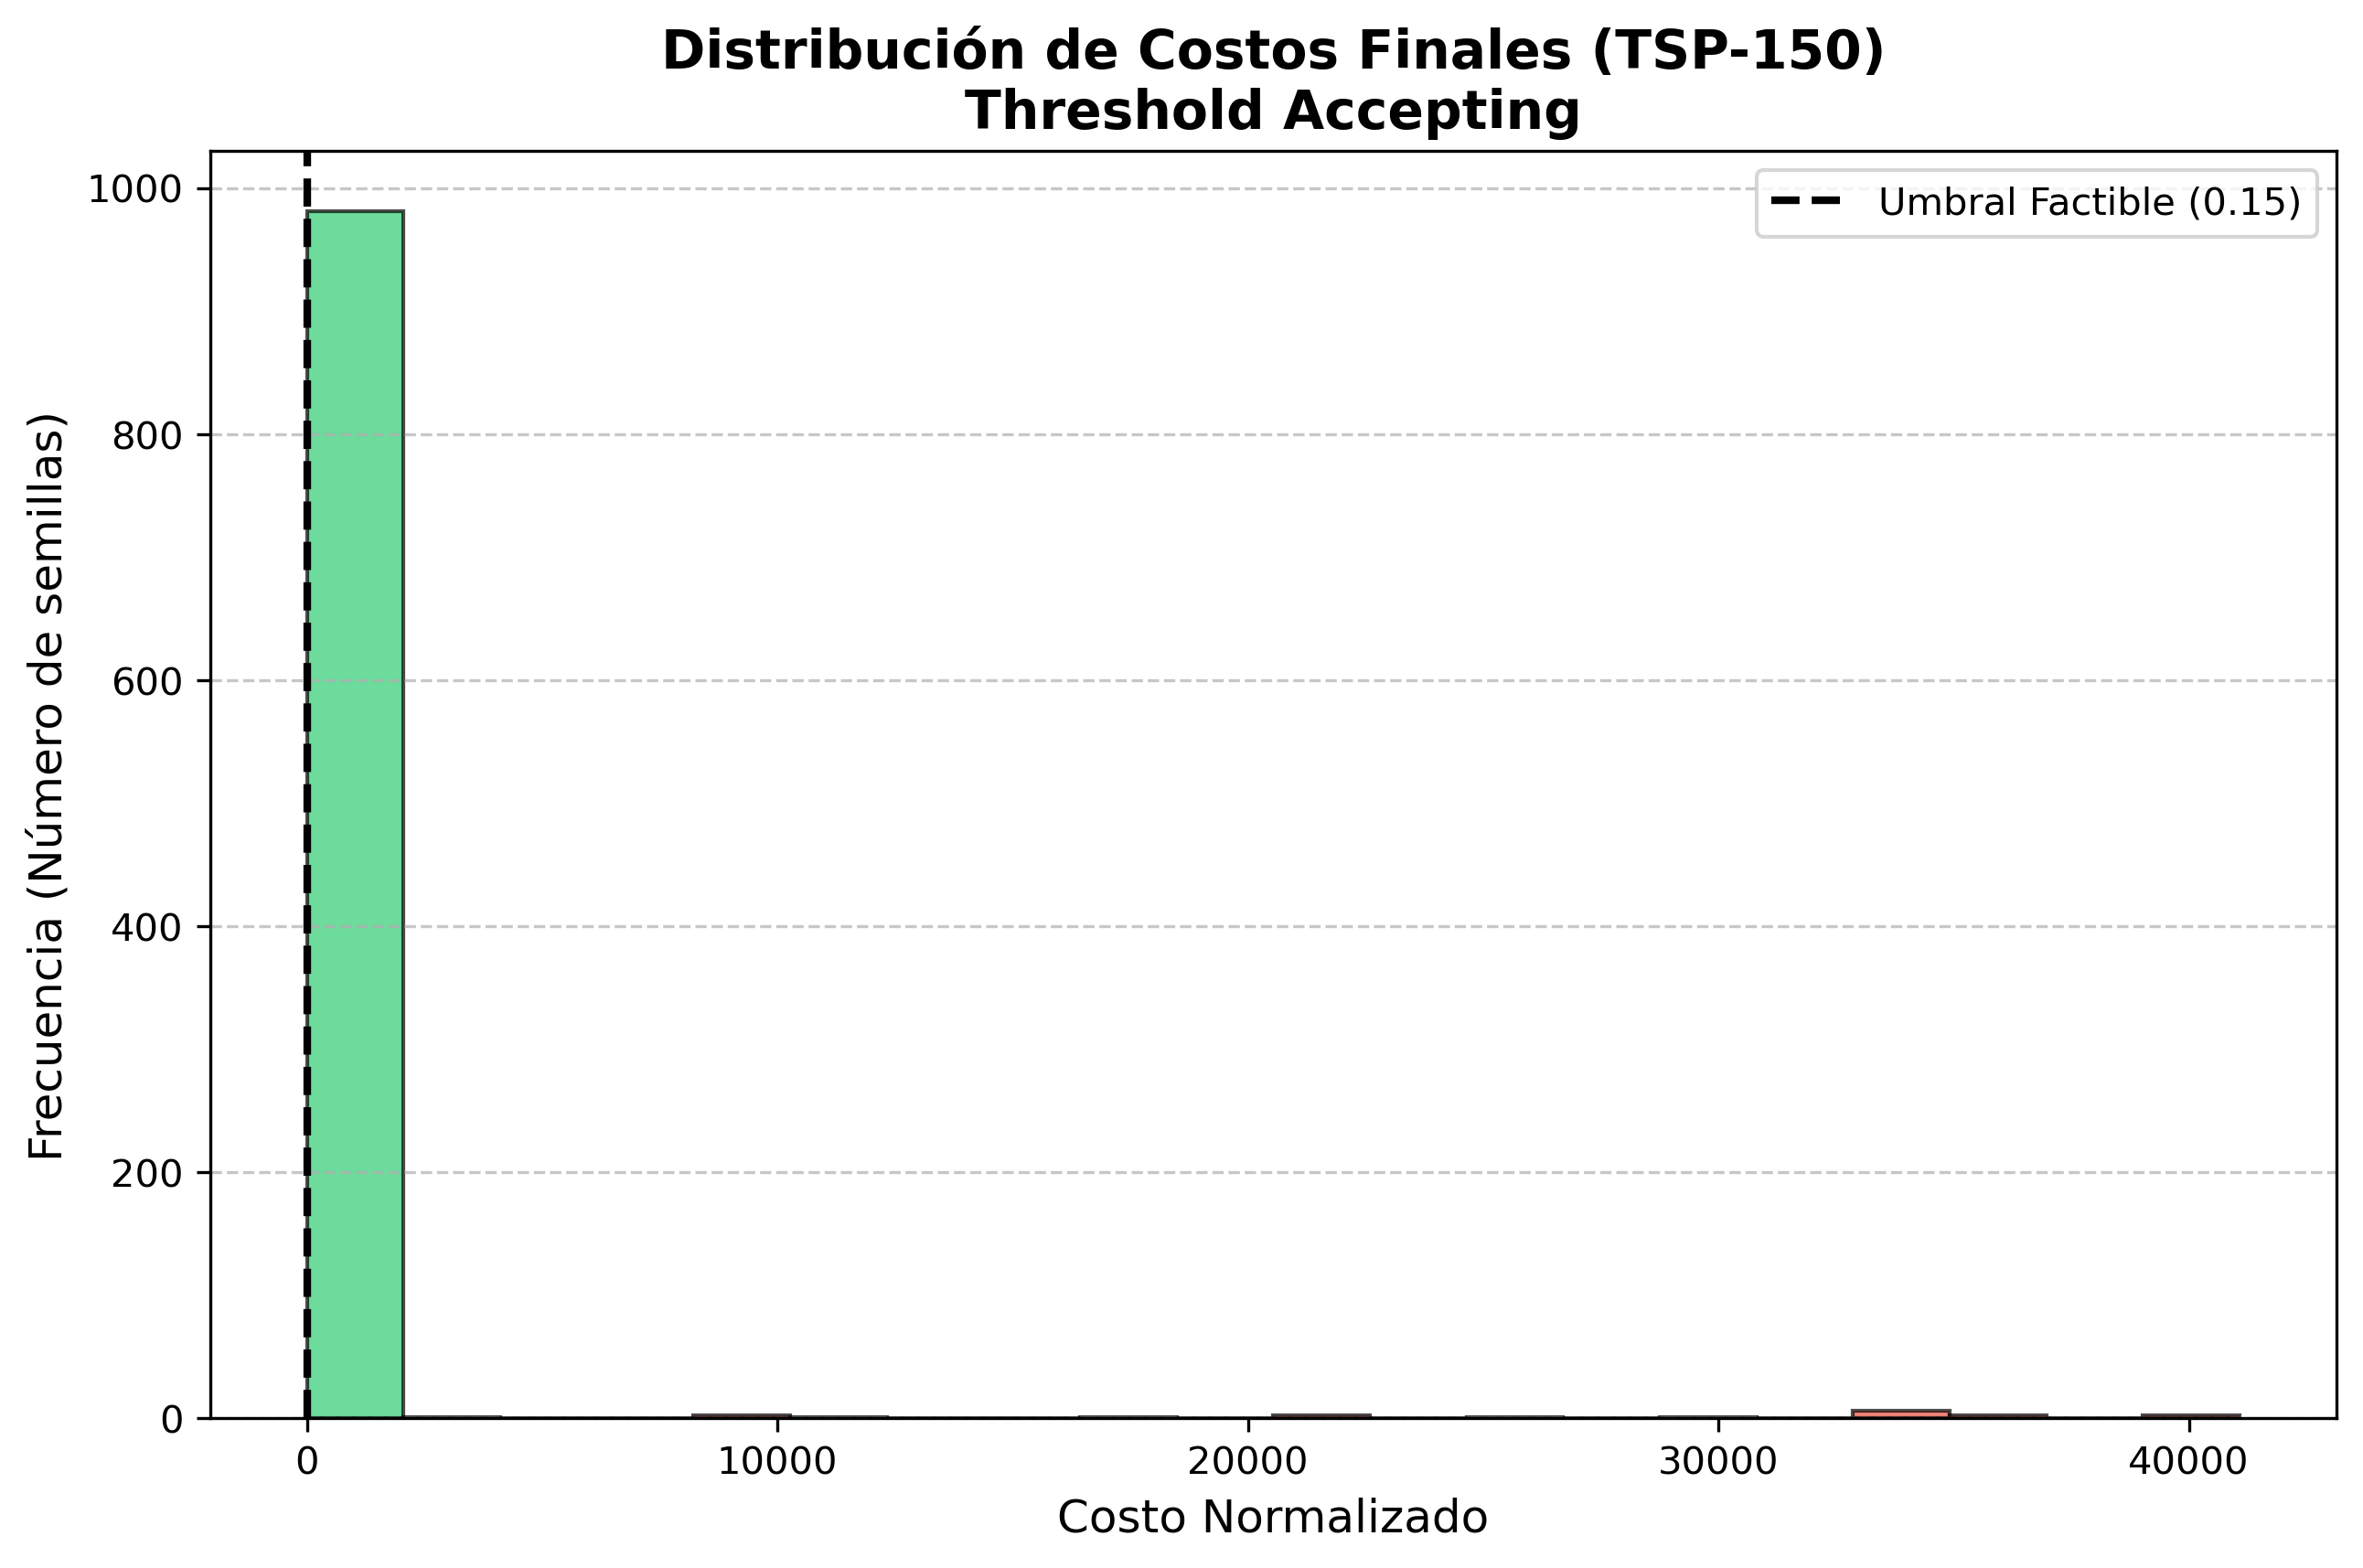
\includegraphics[width=0.8\textwidth]{histograma_tsp150.png}
    \caption{Distribución de los costos finales sobre 1,000 ejecuciones (semillas) de la 0 a la 1000 para la instancia TSP-150. El umbral objetivo de 0.15 está marcado en línea punteada.}
    \label{fig:histograma}
\end{figure}

Como se observa, la gran mayoría de las semillas convergieron de manera consistente hacia el valle de atracción objetivo, logrando costos por debajo de 0.15. Las corridas descartadas o no factibles son estadísticamente marginales.

\newpage
Además, la mejor solución encontrada fue evaluada en 0.139402 con la semilla 614, con la secuencia de IDs de ciudades: \{494, 495, 167, 328, 326, 1037, 169, 1073, 330, 819, 655, 818, 666, 658, 166, 822, 74, 1001, 297, 980, 336, 840, 350, 670, 327, 511, 504, 500, 825, 20, 660, 510, 343, 985, 674, 334, 999, 8, 662, 331, 349, 1003, 11, 164, 25, 492, 491, 499, 347, 489, 4, 174, 817, 23, 176, 668, 352, 978, 5, 6, 1004, 351, 981, 988, 165, 3, 333, 990, 353, 27, 991, 185, 22, 676, 490, 344, 653, 654, 26, 820, 345, 332, 181, 14, 982, 187, 816, 678, 823, 7, 507, 184, 667, 656, 2, 173, 673, 665, 163, 172, 182, 496, 19, 839, 815, 9, 1, 829, 661, 832, 663, 657, 508, 986, 505, 168, 329, 509, 493, 979, 837, 995, 984, 501, 17, 444, 826, 244, 339, 1038, 12, 828, 502, 340, 675, 186, 520, 16, 671, 179, 652, 1075, 483, 512, 821, 75, 346, 183, 77, 171\}. Este es el recorrido de dicha solución:

\begin{figure}[H]
    \centering
    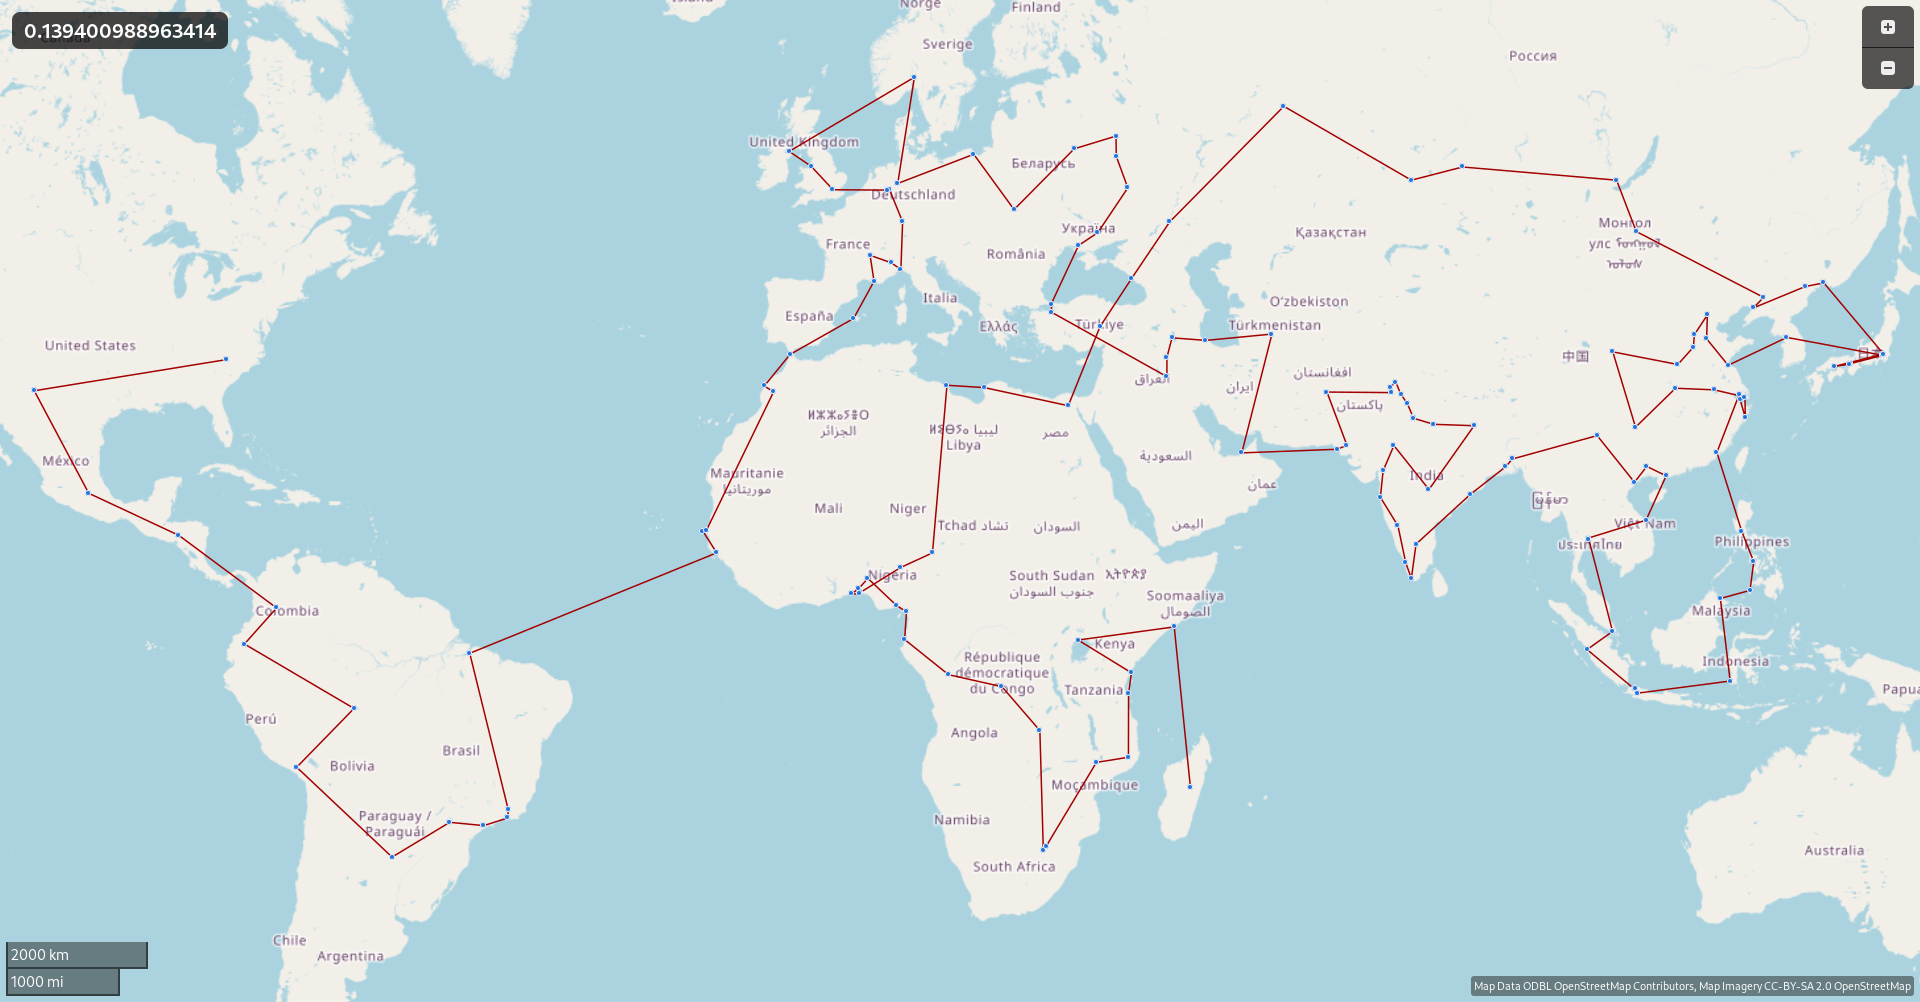
\includegraphics[width=0.8\textwidth]{recorrido.png}
    \caption{Mapa del recorrido.}
    \label{fig:recorrido}
\end{figure}

\section{Conclusiones}
La implementación de la Aceptación por Umbrales con una condición de paro basada en la fluctuación del costo promedio de lotes demostró ser robusta y determinista. La integración de técnicas de ingeniería de software como la mutación \textit{in-place} compensó ampliamente la exploración intensiva en cada meseta térmica. Fue factible alcanzar un costo inferior a 0.15 para la instancia de 150 ciudades, evidenciando la eficacia del método propuesto por Dueck y Scheuer en espacios de búsqueda de alta complejidad. No obstante, el sistema es susceptible de mejora continua, siendo la ausencia de procesamiento paralelo a nivel de hilos y la ausencia del barrido para cerciorarnos de que la solución final sea la mejor a nivel local limitantes importantes a considerar en futuras extensiones del proyecto.

\begin{thebibliography}{9}

\bibitem{dueck1990} 
Dueck, G., \& Scheuer, T. (1990). 
\textit{Threshold accepting: A general purpose optimization algorithm appearing superior to simulated annealing}. 
Journal of Computational Physics, 90(1), 161-175.

\bibitem{michalewicz2000} 
Michalewicz, Z., \& Fogel, D. B. (2000). 
\textit{How to Solve It: Modern Heuristics}. 
Springer-Verlag.

\end{thebibliography}

\end{document}
